\documentclass[english]{uzhpub}
\usepackage[T1]{fontenc}
\usepackage[latin9]{inputenc}

\usepackage[separate-uncertainty]{siunitx}
\sisetup{
    range-units = single,       % \SIrange soll die Einheit nur einmal anzeigen
    list-units  = repeat,       % \SIlist soll die Einheit wiederholen
}


%% erlaubt Listen einfacher zu formatieren (bietet nosep für kompakte Listen)
\usepackage{enumitem}
%% erlaubt hübsche Tabellen über mehrere Seiten, beinhaltet booktabs (\toprule, \midrule, ...)
\usepackage{ctable}
%% ermöglicht farbigen Text ({\color{red} ...})
\usepackage{xcolor}

%% erweiterte Funktionalität für Formeln (Pakete der American Mathematical Society)
\usepackage{amsfonts,amsmath,amsthm,amssymb}

\usepackage{graphicx}
%% ermöglicht Bilder und Tabellen am eingegebenen Ort zu platzieren ([H])
\usepackage{float}
%% ermöglicht Unter-Bilder in einer figure-Umgebung
\usepackage{subfig}
%% Grafik-Dateien werden in den folgenden Ordnern gesucht
\graphicspath{{img/}}
%% Grafikdateien haben die folgenden Endungen (höchste Priorität zu erst)
\DeclareGraphicsExtensions{.pdf,.png,.jpg}

%% Vertikaler Abstand zwischen Absätzen, Beginn eines Absatzes nicht einrücken
\usepackage{parskip}
% \setlength{\parskip}{0.6em}   % Vertikaler Abstand zwischen Absätzen anpassen
% \setlength{\parindent}{0em}   % Einrück-Abstand anpassen

%% zeige Labels im Seitenrand. Dies ist praktisch um Verweise zu kontrollieren
\usepackage[final]{showkeys} % die Option 'final' deaktiviert die Ausgabe von showkeys


%% Ermöglicht Links im PDF
%%   sollte möglichst spät in der Präambel geladen werden
\usepackage[
 pdftex,                        % wir verwenden pdftex/pdflatex
 bookmarks=true,                % wir wollen auch im PDF-Reader ein Inhaltsverzeichnis
 bookmarksdepth=3,              % das Inhaltsverzeichnis soll 3 Tiefen enthalten
 colorlinks=true,               % Linktexte sollen Farbig sein
 linkcolor=black,               % Links innerhalb des Dokuments bleiben schwarz
 citecolor=black,               % Links zu Quellenangaben bleiben ebenfalls schwarz
 urlcolor=blue,                 % URL-Linktexte sollen blau dargestellt werden
%  pdfborder={0 0 0}              % Links im PDF erhalten keinen Rahmen, nur nötig wenn colorlinks=false
]{hyperref}


\begin{document}

%% Titelei
\title{Masterthesis: analysis of $B$ $\rightarrow$ $K^{*}$ $\mu$ $\mu$ decay}

\subtitle{Supervisors: Prof. Dr. Nicola Serra, Dr. Marcin Chzsaszcz}

\author{Author: Oliver Dahme}

%\date{Date}

\maketitle



%% Addpart entspricht dem "Kapiteltitel"
\addpart{Abstract}

\begin{abstract}
  Here comes the abstract
\end{abstract}

%\addpart{Introduction}

\addpart{Introduction}

\section{$B$ $\rightarrow$ $K^{*}$ $\mu$ $\mu$ decay}
The Decay is a flavor changing neutral current (FCNC) with four charged particles in the final state: \\
The $K^+$ and $\pi^-$ from the $K^{*}$ decay and two leptons from the loop or box digrams:
\begin{figure}[H]
  \centering
  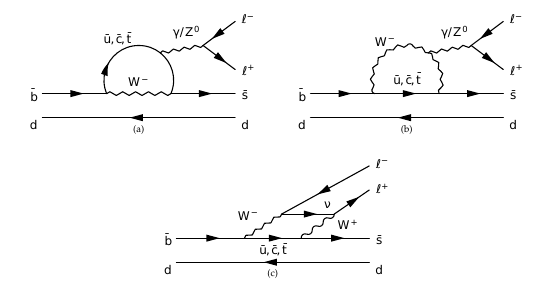
\includegraphics[width=0.8\linewidth]{KstarFeynman}
  \caption{Feynman diagrams for decay $B_d$ $\rightarrow$ $\mu^+$ $\mu^-$ at lowest order}
  \label{fig:Feynman}
\end{figure}
The kinematics of the decay are defined by the three angels $\theta_K$, $\theta_L$ and $\phi$:
\begin{figure}[H]
  \centering
  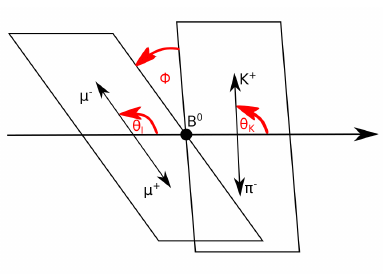
\includegraphics[width=0.6\linewidth]{angels}
  \caption{kinematic variables of the decay $B^0$ $\rightarrow$ $K^{*0}$ $\mu$ $\mu$}
  \label{fig:angels}
\end{figure}


\section{The LHCb Experiment}
The Large Hadron Collider beauty experiment (LHCb) is one of four large experiments based at the CERN laboratory near Geneva in Switzerland. It is part of the Large Hadron Collider (LHC), a proton-proton accelerator and collider located in a vast unterground tunnel with 26.7 km circumference beneath the Swiss-French countryside.
The other three experiments are CMS and ATLAS which are dedicated to a wide range of physics and have therefor very large detectors. ALICE investigates quark-gluon plasma and therefor needs geavy ion collisions, instead of proton collisions. \\
The protons in the LHC have a kinetic energy of 7 TeV, which allows a collision energy, in the LHCb detector, of 13 TeV. In the year 2016 the LHCb had a recorded luminosity of $\SI{1906}{pb^{-1}}$. For this thesis $\SI{2280}{pb^{-1}}$ of data, collected at LHCb during the years 2011 to 2016 are used.
LHCb is dedicated to falvour physics. It therefor investigates rare decays and CP violation in beauty and charm hadrons.

\begin{figure}[H]
  \centering
  \includegraphics[width=1.0\textwidth]{{{LHC_default}}}
  \caption{CERN's Accelerator Complex.\cite{bib:lhc_img} The protons get injected in the lineare accelerator LINAC2. Then they get pre-accelerated in 3 synchrotons (BOOSTER,PS,SPS) where the protons reach a kinetic energy of 450 GeV. That is the entering energy of the LHC which accelerates them futher up to 7 TeV, before they collide at the four detectors: CMS, ATLAS, LHCb and ALICE.}
  \label{fig:lhc}
\end{figure}



\subsection{The LHCb Detector}
The LHCb Detector has a fix target geometry, because beauty hadrons are manily produced at small angeles with respect to the beam pipe.

\begin{figure}[H]
  \centering
  \includegraphics[width=1.0\textwidth]{{{lhcb_detector}}}
  \caption{Basic layout of the LHCb detector \cite{bib:lhcb_detector}. The interaction point is inside the vertrex detector and the beam pipe passes through the center. The different subdetecors are the two Ring Imaging Cherenkov Detecors (RICH1 and RICH2), the tracking stations (TT and T1 to T3), the scintillator pad detector (SPD), the preshower electromagnetic calorimeter (ECAL), the hadronic calorimeter (HCAL) and the muon stations (M1-M5). }
  \label{fig:lhcb_detector}
\end{figure}


\textbf{VErtex LOcator (VELO) \cite{bib:velo} :} Velo picks out B mesons from the multitude of other particles produced. This is a complex task since B mesons have very short livetimes spent colse to the beam. The VELO's silicon detecor elements must be placed at a distance of just five milimetres to the interaction point. To prevent damage to the detector during beam injection and stabilization it is mechanically moved to a safe distance. Velo measures B mesons indirectly be detecting its decay particles, nevertheless it has a resolution of $\SI{10}{microns}$. . \\
\textbf{Ring Imaging Cherenkov (RICH) detectors \cite{bib:rich} :} The RICH detectors meeasure the emission of Cherenkov radiation, which happens when a charged particle passes through a medium faster than light does. It is a similar effect like the sonic boom a aircraft produces by breaking the sound barrier. The shape of the light cone depends on the particle's velocity, enabling the detector to determine its speed.  \\
\textbf{Magnet \cite{bib:mag} :} The big magnet of the LHCb experiment weights 27 tonnes ands is mounted inside a 1,450 tonne steel frame. This powerful magnet forces all charged particels to change there trajectory. By examining the curvature of the path one can calculate its momentum.  \\
\textbf{Trackers \cite{bib:trac} :} The LHCb's tracking system consists of a series of four large rectangular stations, each covering an area of $\SI{40}{m^2}$. While flying through this area charged particles will leave a trace, therefor one can estimate the trajectory of a particle. The trajectory is used to link the signals left in other detecor elements to the corresponding particle. In LHCb two different tracker technologies are used: The silicon tracker placed close to the beam pipe, uses silicon microstripes. If a charged particle passes such a stripe it collides with the silicon atoms, liverating electrons and creating an electric current, which is then recorded. The outer tracker situated further from the beam pipe consists of gas-filled tubes. The gas ionizes when a charged particle hits a gas molecules, producing electrons. These reach an anode wire situated in the centre of each tube. The position of the track is found by timing how long it takes electrons to reach it. \\
\textbf{Calorimeters \cite{bib:calo} :} Calorimeters stop particles as they pass through, measuring the amount of energy lost. In LHCb there are two different types: The elctromagnetic calorimeter responsible for light particles like electrons and photons and the hadronic calorimeter responsible for heavier particles containing quarks. Both have a sandwich-like structure, with alternating layers of metal and plastic plates. If a particles hits a metal plate it produces a shower of secondary particles. These will excite polystyrenne molecules in the plastic plates, which then emit ultraviolet light. The energy lost by the particle in the metal plate is propoertional to the amount of UV light produced in the platic plates. \\
\textbf{Muon System \cite{bib:muonSys} :} The muon system consistes of 5 rectangular stations, which cover an area of $\SI{435}{m^2}$. Each station has chambers filled with three gases: carbon dioxide, argon and tetrafluoromethane. Passing muons react with the mixture and electrodes detect the result.


\subsection{The LHCb trigger system}
The rate of events at the LHCb interaction point is $\SI{40}{MHz}$. But the rate to have a B meson contained in the detector is $\SI{15}{kHz}$. But the offline computing power just allows $\SI{2}{kHz}$ to be recorded. The LHCb trigger system aims to 'fill' this $\SI{2}{kHz}$ with intresting B decays and important control decays like $J/ \psi$ decays. The trigger has two levels: \\
The \textbf{Level Zero (L0)} trigger reduces the beginning $\SI{40}{MHz}$ to $\SI{1}{MHz}$. To get this high rate it can only rely on fast sub-detectors as the calorimeters and the muon system. The L0 trigger looks for events with high transverse momentum with respect to the patrticle beam axis (pT), because particles from a B decay have this attribute, since B Mesons are always produced almost parallel to the beam axis.
In addition the L0 trigger performs a simplified vertex reconstruction with the signal of two silicon layers of the VELO to identifie events with multple proton-proton collisions. They are rejected because for this kind of events its much more difiicult to reconstruct B meson decays, since it is harder to distinguish primary and secondary vertex of the B decay. \\
The \textbf{High Level Trigger (HTL)} is an algorithm that runs on a farm of 1000 16-core computers. It has two stages: HLT1 which reduces the event rate to a few tens of kHz and HLT2 which reduces the rate to the $\SI{2}{kHz}$ which are recorded. HLT1 gets all the candidates of the L0 trigger and uses the full detector information on them to search for particles with a high impact parameter with respect the proton-proton collision. These particles are most likly decay products from B mesons, because of its relatively long life-time. They typically fly 1 cm away from the collision before decaying resulting in a high impact parameter for the decay products. HLT2 does a complete reconstruction of the events. It starts with the track of the VELO and connects them to the tracks in the other sub-detectors. Most important are displaced vertices, since they are strong indicator for B decays. The selection is devided into two parts. The inclusive selection searches for resonance decays like $D^*$ or $J/ \psi$. The exclusive selection is desigened to provide the highest possible efficiency to fully reconstruct B decays of interest. It therfor uses all information available such as mass and vertex quality and intermediate resonances.

\section{Analysis}

\subsection{Classification}

\subsubsection{Introduction}

To eliminate combinatorial background Machine Learning algorithms called classifiers are used. They can seperate data into two or more parts, depending on certain parameters.For example sperating colors depending on their share of magenta, cian and yellow. But first they need to be trained on so called labeled data. In a labeled data set it is known which entrie corresponds to which category, like colors. While training the algorithm will learn so sperate data into the pre defined categories. That is the reason it is called Machine learning. In this thesis the classfication should seperate signal from combinatorial background. \\
To do so Monte Carlo data which contains only $B$ $\rightarrow$ $K^{*}$ $\mu$ $\mu$ decays is labeled with probability $1$ to be signal. Then it is merged with real data and used to train the classifiers. But since the classification becomes naturally biased if the data to classify is the same as the training data, a technique called K-folding is used. K-folding seperates the data Monte Carlo mix into several parts called folds. To classify one fold all the other folds are used for training. After iterating over all the folds one has a complety classified data set without any bias. \\

\subsubsection{classifiers test}
In this thesis the classifiers themselves are used as a black box and are not explained further.
First the following list of classifers where tested and compared in terms of perfomance:
\begin{itemize}
  \item Ada Boost
  \item uGB + knnAda
  \item uBoost
  \item uGB + Fl
  \item xgb
  \item sk\_bdtg
  \item sk\_bdt
\end{itemize}
The test was performed with 30000 events from the 2016 LHCb $B$ $\rightarrow$ $K^{*}$ $\mu$ $\mu$ data and 10000 events from the Monte Carlo simulation. The following list of parameters are used in brackets are the names of the parameters in the root files.
\begin{itemize}
  \item Decay vertex location for reconstructed particles (ENDVERTEX)
  \item Primary vertex location (OWNPV)
  \item Impact parameter (IP\_OWNPV)
  \item Flight distance (FD\_OWNPV)
  \item The cosine of the angle between primary vertex and decay vertex and recorded momentum (DIRA\_OWNPV)
\end{itemize}
To compare the different classifiers the ROC curves and the correlations to the kinematic variabels of the decay (see \ref{fig:angels}) are used. Since the curves for the different folds all look alike only one is presented here. One can find the other in the appendix \ref{app:roc} \ref{app:corr}.

\subsection{SPlot}
SPlot is a tecnique to subtract the exponatial background from the signal.



\subsection{Reweighting}






\begin{thebibliography}{100}
  \addcontentsline{toc}{section}{Bibliography}

  \bibitem{bib:lhc_img} CERN Accelerator Complex,
  \url{http://www.stfc.ac.uk/research/particle-physics-and-particle-astrophysics/large-hadron-collider/cern-accelerator-complex/}

  \bibitem{bib:lhcb_detector} Science and Technology Facilities Council article about LHCb ,
  \url{https://www.ppd.stfc.ac.uk/Pages/LHCb.aspx}

  \bibitem{bib:velo} VELO description,
  \url{http://lhcb-public.web.cern.ch/lhcb-public/en/Detector/VELO2-en.html}

  \bibitem{bib:rich} RICH description,
  \url{http://lhcb-public.web.cern.ch/lhcb-public/en/Detector/RICH2-en.html}

  \bibitem{bib:mag} Magnet description,
  \url{http://lhcb-public.web.cern.ch/lhcb-public/en/Detector/Magnet2-en.html}

  \bibitem{bib:trac} Tracker description,
  \url{http://lhcb-public.web.cern.ch/lhcb-public/en/Detector/Trackers2-en.html}

  \bibitem{bib:calo} Calorimeters description,
  \url{http://lhcb-public.web.cern.ch/lhcb-public/en/Detector/Calorimeters2-en.html}

  \bibitem{bib:muonSys} Muon system description,
  \url{http://lhcb-public.web.cern.ch/lhcb-public/en/Detector/Muon2-en.html}

\end{thebibliography}

\begin{appendix}
  \section{ROC curves}
  \label{app:roc}

  \section{Learning Curves}
  \label{app:lc}

  \section{Correlation plots}
  \label{app:corr}



\end{appendix}

\end{document}
